
\paragraph{Circuito magnetico con più traferri}
Si realizza un circuito magnetico con tre traferri di sezione $S_1,S_2,S_3$ e 
ampiezze $\delta_1,\delta_2,\delta_3 $ come in figura
\begin{figure}[H]
\centering
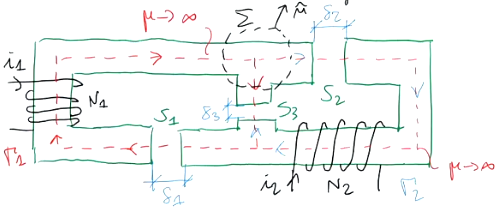
\includegraphics[width = 0.6\linewidth]{circuito_magnetico_traferri}
\end{figure}

Si suppone che la permeabilità nel ferro sia infinita, ci si pone l'obbiettivo di 
determinare i coefficienti di auto e mutua induzione. 
Si orientano delle linee lungo le quali calcolare i flussi, concordi al 
verso di avvolgimento di generatori.

Si applica la legge di Hopkinson
$$
\Phi_J = \iint_{S_j} \vec{B}\cdot\hat{n}dS
$$
$$
\Gamma_1:\ N_1i_1  = \mathcal{R}_3\Phi_3 + \mathcal{R}_1\Phi_1
$$
$$
\Gamma_2:\ N_2i_2 = -\mathcal{R}_3\Phi_3 + \mathcal{R}_2\Phi_2
$$
$$
\mathcal{R}_j =\int_{\text{tubo flusso}} \frac{dl}{\mu_lS_L}=\frac{\delta_j}{\mu_jS_j}
$$

In un circuito magnetico, come in quello elettrico, esistono i ``nodi'', ossia
superfici chiuse che tagliano il circuito magnetico in regioni dove sono presenti
più flussi come la regione $\Sigma$ in figura.

$$
\oiint_\Sigma\vec{B}\cdot\hat{n}dS \simeq -\Phi_1 + \Phi_2 +\Phi_3 = 0
$$
È importante ricordare di orientare i flussi concordemente alla superficie 
$\Sigma$ sul nodo e utilizzare i segni corretti se questi risultano entranti
o uscenti, così come si considerano le correnti in un nodo secondo la 
LKC.

Il sistema di equazioni che risolve il problema è dunque
$$
\begin{cases}
N_1i_1  = \mathcal{R}_3\Phi_3 + \mathcal{R}_1\Phi_1\\
N_2i_2 = -\mathcal{R}_3\Phi_3 + \mathcal{R}_2\Phi_2\\
-\Phi_1 + \Phi_2 +\Phi_3 = 0
\end{cases}
$$

Si può realizzare un equivalente circuitale elettrico, si utilizza un generatore
di tensione per ogni forza magnetomotrice, si sostituisce ogni traferro con un resistore
.
\begin{figure}[H]
\centering
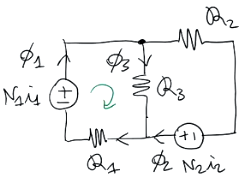
\includegraphics[width=0.4\linewidth]{circuito_magnetico_traferri_equivalente}
\end{figure}
Il circuito si può risolvere con i classici metodi dei circuiti elettrici.
Si applica ad esempio il PSE spegnendo il secondo generatore
$$
\Phi_1' = \frac{N_1i_1}{\mathcal{R}_1 + \mathcal{R}_2 // \mathcal{R}_3}
\qquad
\Phi_2' = \Phi_1' \frac{\mathcal{R}_3}{\mathcal{R}_2+\mathcal{R}_3}
$$
Ora si spegne il generatore $N_1i_1$
$$
\Phi_1'' = \Phi_2'' \frac{\mathcal{R}_3}{\mathcal{R}_3 + \mathcal{R}_1}
\qquad
\Phi_2'' = \frac{N_2i_2}{\mathcal{R}_2+\mathcal{R}_1//\mathcal{R}_3}
$$
Si possono ora sommare i contributi
\begin{align*}
&\Phi_1 = \Phi_1' + \Phi_1''\\
&\Phi_2 = \Phi_2' + \Phi_2''
\end{align*}
Si calcolano i coefficienti di auto e mutua induzione utilizzando le definizioni
\begin{align*}
L_1 &= \left.\frac{\Phi_1^c}{i_1}\right|_{i_2 = 0} = \frac{N_1\Phi_1'}{i_1} = \frac{N_1^2}{\mathcal{R}_1 + \mathcal{R}_2//\mathcal{R}_3}\\
M_{21} &= \left.\frac{\Phi_2^c}{i_1}\right|_{i_2 = 0} = \frac{\Phi_2' N_2}{i_1} =
\frac{N_1N_2}{(\mathcal{R}_1+\mathcal{R}_2//\mathcal{R}_3)}\frac{\mathcal{R}_3}{(\mathcal{R}_2\mathcal{R}_3)}\\
L_2 &= \left.\frac{\Phi_2^c}{i_2}\right|_{i_1 = 0} = \frac{\Phi_2''N_2}{i_2} = \frac{N_2^2}{\mathcal{R}_2+\mathcal{R}_1//\mathcal{R}_3}\\
M_{12} &= \left.\frac{\Phi_1^c}{i_2}\right|_{i_1 = 0} = \frac{N_1\Phi_1''}{i_2} = \frac{\mathcal{R}_3}{\mathcal{R}_3+\mathcal{R}_1}\frac{N_2N_1}{\mathcal{R}_2+\mathcal{R}_1//\mathcal{R}_3}
\end{align*}
Si vede quindi che $M_{21} = M_{12}$ e che $L_1L_2 \geq M^2$ per la condizione di fisica
realizzabilità.
\newpage
\subparagraph{Esempio numerico}
\begin{align*}
&N_1 = 100, \quad N_2 = 200\\
&\delta_1 = \delta_2=\delta_3 = \SI{2}{\milli\meter} \\
& S_1 = \SI{25}{\milli\meter^2},\quad\ S_2 = \SI{49}{\milli\meter^2},\quad\ S_3 = \SI{36}{\milli\meter^2}\\
&L_1 = \SI{0.12}{\milli\henry},\quad L_2 = \SI{0.68}{\milli\henry}, \quad  M = \SI{0.14}{\milli\henry}
\end{align*}
\subparagraph{Circuito magnetico non lineare}
Si consideri un circuito con un solo traferro come ad esempio un giogo a C, con un avvolgimento sul braccio sinistro di $N$ spire, si stabilisce la linea media sull'asse
del tubo di flusso, sulla quale vengono prese le dimensioni caratteristiche dell'oggetto.
\begin{figure}[H]
\centering
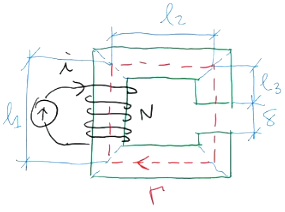
\includegraphics[width = 0.4\linewidth]{circuito_magnetico_non_lineare}
\end{figure}

Si suppone che il materiale sia ferro dolce con ciclo stretto e saturazione da un certo 
punto in poi.

Può essere necessario calcolare varie grandezze come
le amperspire ($Ni$) necessarie a produrre una certa induzione $B_t$ al traferro
(ad esempio per il dimensionamento di un elettromagnete).
Si applica la legge di Ampere
$$
\oint_\Gamma \vec{H}\cdot\hat{t}dl = Ni \simeq H_1l_1 + 2H_2l_2 +2H_3l_3+\delta \frac{B_t}{\mu_0}
$$

In questo caso l'oggetto in analisi non è un tubo di flusso per $\vec{B}$ a causa della 
non linearità della permeabilità magnetica quindi $\Phi_t \neq \Phi_1 \neq \Phi_2 \neq \Phi_3 $ e in genere si definisce un coefficiente minore di uno a seconda della geometria 
che paragona i flussi, determinati sperimentalmente e tabellati.
$$
\Phi_1 = k_1 \Phi_t,\quad \Phi_2 = k_2 \Phi_t,\quad \Phi_3 = k_3 \Phi_t
$$
$$
\Phi_t = B_tS_t \Rightarrow \begin{aligned}
&\Phi_1 = k_1 B_t S_t = B_1S_1\\
&\Phi_2 = k_2 B_t S_t = B_2S_2\\
&\Phi_3 = k_3 B_t S_t = B_3S_3
\end{aligned}
$$
Da queste equazioni si ricavano i campi $B_1,\ B_2,\ B_3$ e rispettivamente i campi
$\vec{H}$ sfruttando la permeabilità delle varie sezioni del giogo, queste sono 
diverse e cercano di tenere in considerazione la non linearità del sistema o meglio
di una linearità a tratti per ogni giogo.

Sostituendo i valori ottenuti nell'equazione della geometria
$$
\frac{B_1}{\mu_1}l_1 + 2\frac{B_2}{\mu_2}l_2 + 2\frac{B_3}{\mu_3}l_3 + \frac{\delta B_t}{\mu_0} = Ni
$$
Si può dunque calcolare $Ni$ e risolvere il problema.

Si affronta ora il problema inverso, data la forza magnetomotrice si vuole determinare
l'induzione al traferro.

La legge di Ampere è sempre valida
$$
H_1l_1 + 2H_2l_2 +2H_3l_3 + \frac{\delta B_t}{\mu_0} = Ni
$$

Si suppone invece di trascurare le dispersioni di flusso nei gioghi
$$
\Phi_t = \Phi_1 = \Phi_2 = \Phi_3 = B_tS_t
$$
$$
\begin{aligned}
&\Phi_1 = B_1S_1 = B_tS_t\\
&\Phi_2 = B_2S_2 = B_tS_t\\
&\Phi_3 = B_3S_3 = B_tS_t
\end{aligned}
\Rightarrow
\begin{aligned}
&B_1 = B_t\frac{S_t}{S_1} \\
&B_2 = B_t\frac{S_t}{S_2}\\
&B_3 = B_t\frac{S_t}{S_3}
\end{aligned}
$$

Si suppone di descrivere la caratteristica del materiale come una curva $B = \mathcal{B}(H)$ assegnata.
Per ricavare $H_1$ va invertita la funzione
$$
\begin{aligned}
&H_1 = \mathcal{B}^{-1} \left(B_t\frac{S_t}{S_1}\right)\\
&H_1 = \mathcal{B}^{-1} \left(B_t\frac{S_t}{S_2}\right)\\
&H_1 = \mathcal{B}^{-1} \left(B_t\frac{S_t}{S_3}\right)
\end{aligned}
$$
Sostituendo nella legge di Ampere
$$
\mathcal{B}^{-1}\left(B_t\frac{S_t}{S_1}\right)l_1 + 2\mathcal{B}^{-1} \left(B_t\frac{S_t}{S_2}\right)l_2 + 2\mathcal{B}^{-1} \left(B_t\frac{S_t}{S_3}\right)l_3 + \delta\frac{B_t}{\mu_0} = Ni
$$
Quella ottenuta è un'equazione non lineare nell'incognita $B_t$, vanno ricavati gli zeri
dell'equazione (uno solo se la curva è monotona decrescente).
\subparagraph{Metodo di Newton-Raphson o delle tangenti}
Viene solitamente utilizzato il metodo di \href{https://it.wikipedia.org/wiki/Metodo_delle_tangenti}{Newton-Raphson}, un metodo iterativo con accuratezza arbitraria
basato sulla costruzione delle tangenti.
\begin{figure}[H]
\centering
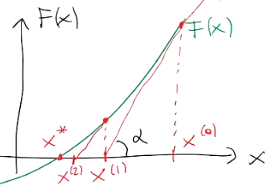
\includegraphics[width = 0.4\linewidth]{metodo_tangenti}
\end{figure}

Si traccia la tangente in un punto arbitrario della funzione e si interseca con
l'asse $x$, si ricava nuovamente la tangente nel punto in cui è ``caduta'' la precedente.
$$
F\left(x^{(0)}\right) = \left(x^{(0)} - x^{(1)}\right) \tan\alpha = \left(x^{(0)} - x^{(1)}\right)F'\left(x^{(0)}\right)
$$
invertendo
$$
x^{(1)} = x^{(0)} - \frac{F\left(x^{(0)}\right)}{F'\left(x^{(0)}\right)}
$$
quindi in generale, si ricava l'iterazione di Newton-Raphson
$$
x^{(k+1)} = x^{(k)} - \frac{F\left(x^{(k)}\right)}{F'\left(x^{(k)}\right)}
$$
È un metodo con velocità di convergenza quadratica, converge sempre se la funzione 
è monotona qualunque sia il punto iniziale. Quando la differenza tra due valori iterati
è inferiore alla precisione richiesta il metodo si arresta $\left|x^{(k+1)}-x^{(k)}\right|< \varepsilon$.
